\documentclass[12pt]{article}
\usepackage[utf8]{inputenc}
\usepackage[english]{babel}
\usepackage[letterpaper, portrait, margin=1in]{geometry}
\usepackage{amsmath}
\numberwithin{equation}{section}
\usepackage{amssymb}
\usepackage{graphicx}
\usepackage{wrapfig}
\usepackage{parskip}
\usepackage{xcolor}
\usepackage{physics}
\usepackage{empheq}
\usepackage{cancel}
\usepackage{hyperref}
\hypersetup{colorlinks = true, urlcolor = blue, linkcolor = red, citecolor = red}
\usepackage{enumerate}
\usepackage{tikz}
\usepackage{float}
\usepackage{tcolorbox}
\usepackage{booktabs}

\usepackage{amsthm}
\theoremstyle{definition}
\newtheorem{theorem}{Theorem}[section]
\newtheorem{definition}[theorem]{Definition}
\newtheorem{claim}[theorem]{Claim}
\newtheorem{proposition}[theorem]{Proposition}
\newtheorem{lemma}[theorem]{Lemma}
\newtheorem{corollary}[theorem]{Corollary}
\newtheorem{conjecture}[theorem]{Conjecture}
\newtheorem{example}[theorem]{Example}


\author{Yi J Zhu}
\title{The $\chi^2$ Distribution and Goodness-of-Fit Tests}
\date{June 30, 2021}

\begin{document}

\maketitle

\section{The $\chi^2$ Distribution }
Suppose $X_1, X_2, \dots, X_k$ are $k$ i.i.d.\footnote{Independent, identically distributed.} standard normal distributions $X_i\sim N(0,1)$. We define the chi-squared distribution with $k$ degrees of freedom as the sum of the squared $X_i$ distributions,
\begin{equation}
		\chi^2_k = \sum_{i=1}^{k} X_i^2
\end{equation}

\subsection{Probability Density Function}

We can determine the chi-squared PDF $f_{\chi^2_k}(x)$ by first writing out its CDF $F_{\chi^2_k}(x)$. If we define,
\begin{equation}
		r_k = \sqrt{\sum_k x_i^2} = \sqrt{x}
\end{equation}
Then CDF is the volume integral of the probability over an $n$-sphere of radius $r_k=\sqrt{x}$,
\begin{figure}[H]
	\centering
	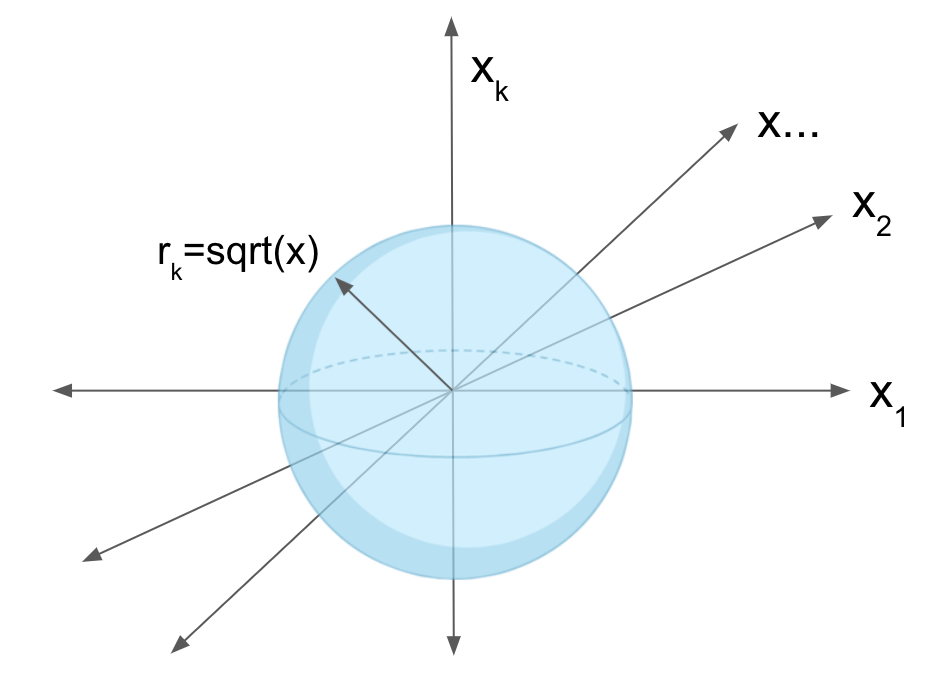
\includegraphics[width=8cm] {sphere}
\end{figure}
\begin{align}
		F(x) &= \int_0^{\sqrt{x} }\left(\prod_k \frac{e^{-x_i^2/2}}{\sqrt{2 \pi}}  \right) A_k(r_k)dr_k\\
		& = \int_0^{\sqrt{x}} \frac{e^{-r_k^2/2}}{(2\pi)^{k/2}}A_k(r_k)dr_k \\
		&= \int_0^x  \frac{e^{-x'/2}}{(2\pi)^{k/2}}A_k\left(\sqrt{x'}\right)\left(\frac{dx'}{2\sqrt{x'}}\right)
\end{align}
Where $A_k(r)$ 	is the surface area of the k-dimensional sphere,
\begin{equation}
		A_k = \frac{2 r^{k-1}\pi^{k/2}}{\Gamma(k/2)}
\end{equation}
Thus,
\begin{equation}
		F(x) = \int_0^x  \frac{e^{-x'/2}}{(2\pi)^{k/2}} \frac{2 x'^{(k-1)/2}\pi^{k/2}}{\Gamma(k/2)} \frac{dx'}{2\sqrt{x'}}
\end{equation}
\begin{equation}
		F(x) = \int_0^x  \frac{e^{-x'/2}}{2^{k/2}} \frac{x'^{(k/2-1)}}{\Gamma(k/2)} dx'
\end{equation}

Now, we obtain the PDF:
\begin{equation}
		f(x) = \dv{F}{x} 
\end{equation}
\begin{equation}
		f_{\chi^2_k}(x) = \frac{e^{-x/2}\ x^{(k/2-1)}}{2^{k/2}\ \Gamma(k/2)} 
\end{equation}

\begin{figure}[H]
	\centering
	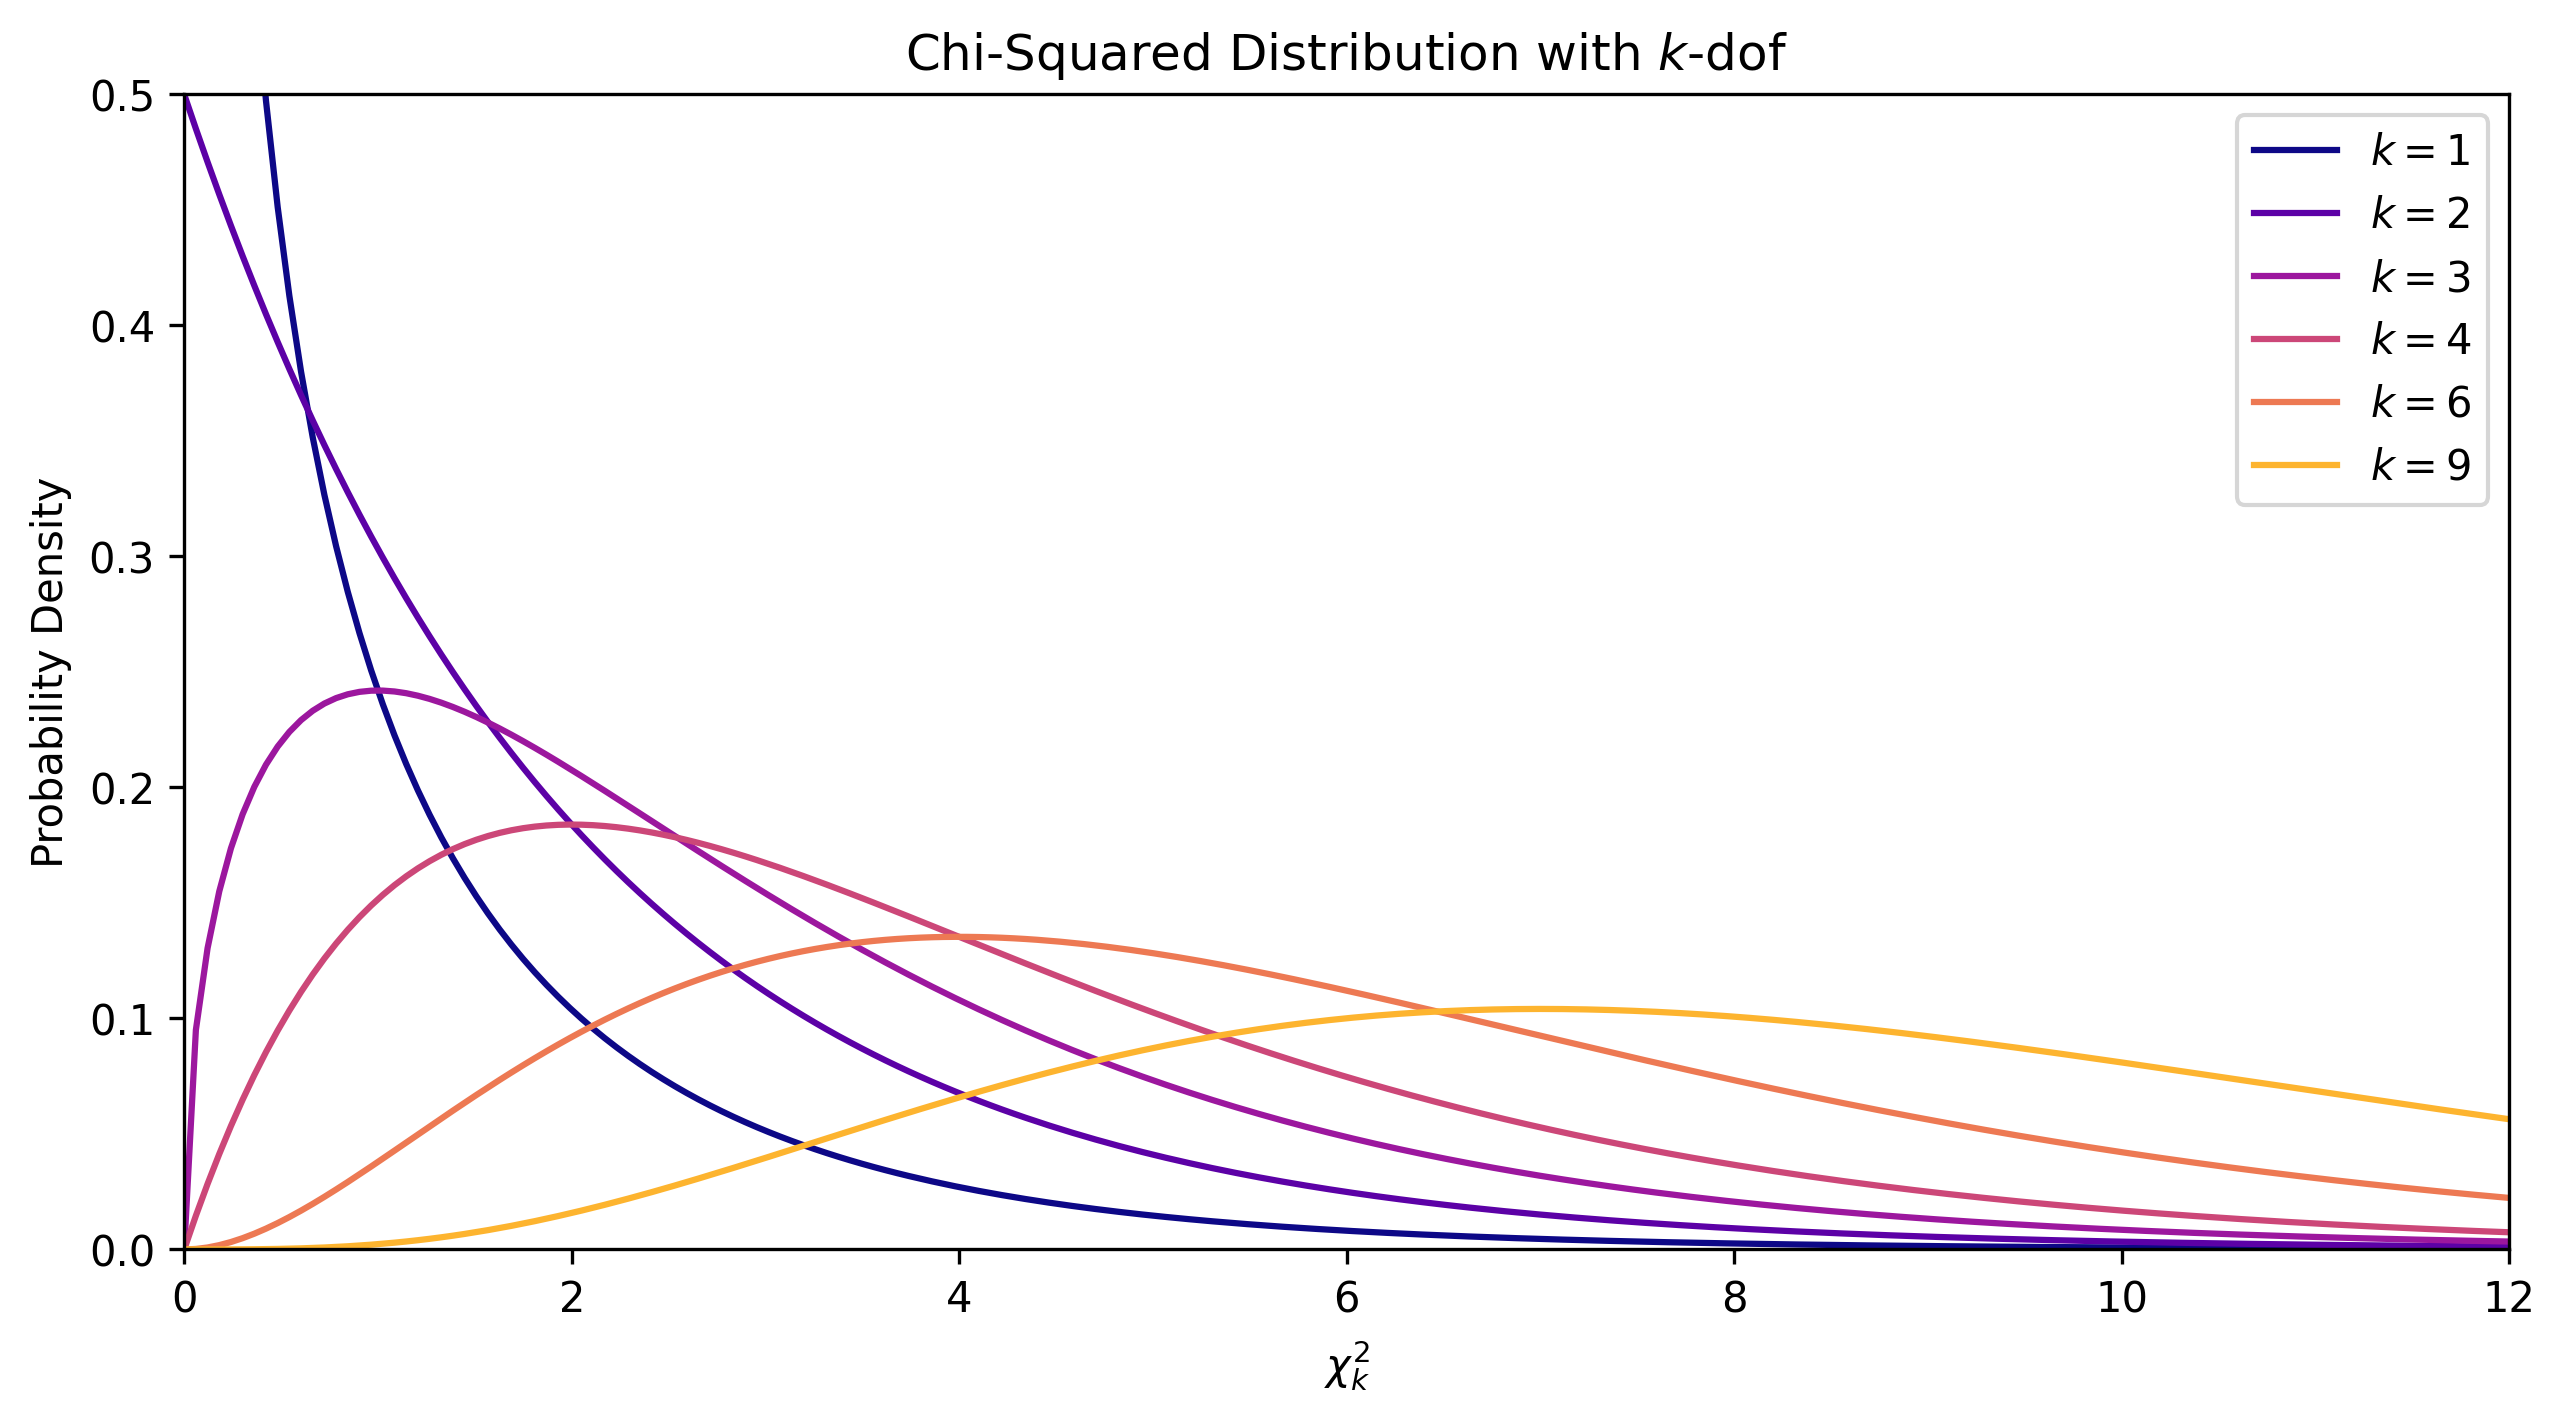
\includegraphics[width=17cm] {pdf}
\end{figure}

\subsection{MGF, Mean, and Variance}

We can calculate the moment generating function of $\chi^2_k$ via brute force,
\begin{align}
		E(e^{t\chi^2}) &= \frac{1}{2^{k/2}\ \Gamma(k/2)}\int_0^{\infty} \left(e^{-x/2}\ x^{(k/2-1)} dx\right) e^{tx}\\
		&=  \frac{1}{2^{k/2}\ \Gamma(k/2)} \int_0^{\infty} x^{(k/2-1)} e^{-x(1/2-t)}dx
\end{align}
for, $u = x(1/2-t)$,
\begin{align}
		E(e^{t\chi^2}) &= \frac{1}{2^{k/2}\ \Gamma(k/2)} \int_0^{\infty} \left(\frac{u}{1/2-t}\right)^{k/2-1}e^{-u} \frac{du}{1/2-t}\\
		&=  \frac{1}{2^{k/2}\ \Gamma(k/2)} \left(1/2-t\right)^{-k/2} \int_0^{\infty} u^{k/2-1}e^{-u}du\\
		&=  \frac{1}{2^{k/2}\ \Gamma(k/2)} \left(1/2-t\right)^{-k/2} \Gamma(k/2)
\end{align}
Thus,
\begin{equation}
		M_{\chi_k^2}(t) = E(e^{t\chi_k^2}) = (1-2t)^{-k/2}
\end{equation}

Now let's calculate the mean,
\begin{equation}
		E(\chi_k^2) = \left.\dv{M_{\chi_k^2}}{t} \right|_{t=0} = \left.\frac{k}{(1-2t)^{k/2+1}}\right|_{t=0}
\end{equation}
\begin{equation}
		E(\chi_k^2) = k
		\label{eq:mean}
\end{equation}

The fact that expectation value is proportional to the degrees of freedom should make sense. We know that $E[\sum_k X_i^2] = \sum_k E(X_i^2) = k E(X_1^2)$. It happens that $ E(X_1^2) = 1$, so the mean is exactly equal to the number of degrees of freedom.

 In other words, the expectation value per degree of freedom is 1. We'll make use of this fact in the next section!

Now, let's calculate the variance. First,
\begin{equation}
		E\left((\chi_k^2)^2 \right) = \left.\dv[2]{M_{\chi_k^2}}{t} \right|_{t=0} =\left. \frac{k(k+2)}{(1-2t)^{k/2+2}}\right|_{t=0} = k^2+2k
\end{equation}
Now,
\begin{equation}
		Var(\chi_k^2) = 	E\left[(\chi_k^2)^2 \right]  - \left[E(\chi_k^2)\right]^2 = k^2+2k - k^2
\end{equation}
\begin{equation}
		Var(\chi_k^2) = 2k
		\label{eq:var}
\end{equation}

\section{Goodness-of-Fit Testing}

There are two types of statistical tests that are commonly performed with the Chi-squared distribution: (1) the reduced Chi-squared test and (2) Pearson's Chi-squared test. The reduced Chi-squared test is used to determine how well a model fits observations assuming Gaussian noise. Pearson's Chi-squared test is a p-value test for a multinomial distribution.

\subsection{Reduced Chi-Squared Test}

Suppose we collect a set of data $ \{x_i, y_i\} $ relating how some variable $y$ relates to variable $x$. Furthermore, let's assume that the sources of error for our measurements are Gaussian, and that the uncertainties for each data point $\{\sigma_i\} $ is known.

We can fit out data to a model $ \hat{y}(\vec{a}; x) $ where $ \vec{a} = (a_1, a_2, \dots, a_m) $ are the fit parameters and $ f_i(x) $ are arbitrary functions of $ x $ that do not involve $ \vec{a} $,
\begin{equation}
		\hat{y}(\vec{a}; x) = \sum_{j=1}^m a_j f_j(x)
		\label{eq:linear}
\end{equation}

If we define the variable $ \chi^2 $ (which we'll justify in a bit),
\begin{equation}
		\chi^2 = \sum_{i=1}^n \left( \frac{y_i-\hat{y}(\vec{a}; x_i)}{\sigma_i}\right)^2
		\label{eq:chi2}
\end{equation}

Then we can determine the optimal fit parameters $\vec{a}$ for our model $\hat{y}(\vec{a}, x)$ by minimizing $\chi^2$. This is known as the method of least squares!\footnote{This is how Scipy's curve fit function operates.}

But how do know how well our fit \textit{fits} our data? We might expect that the smaller the value of $\chi^2$, the smaller the residuals, and the better our fit. This reasoning is correct, but misleading. Instead, we often used the reduced Chi-squares statistic $\chi^2_r$ as a heuristic for how well our model fits the data.

\begin{figure}[H]
	\centering
	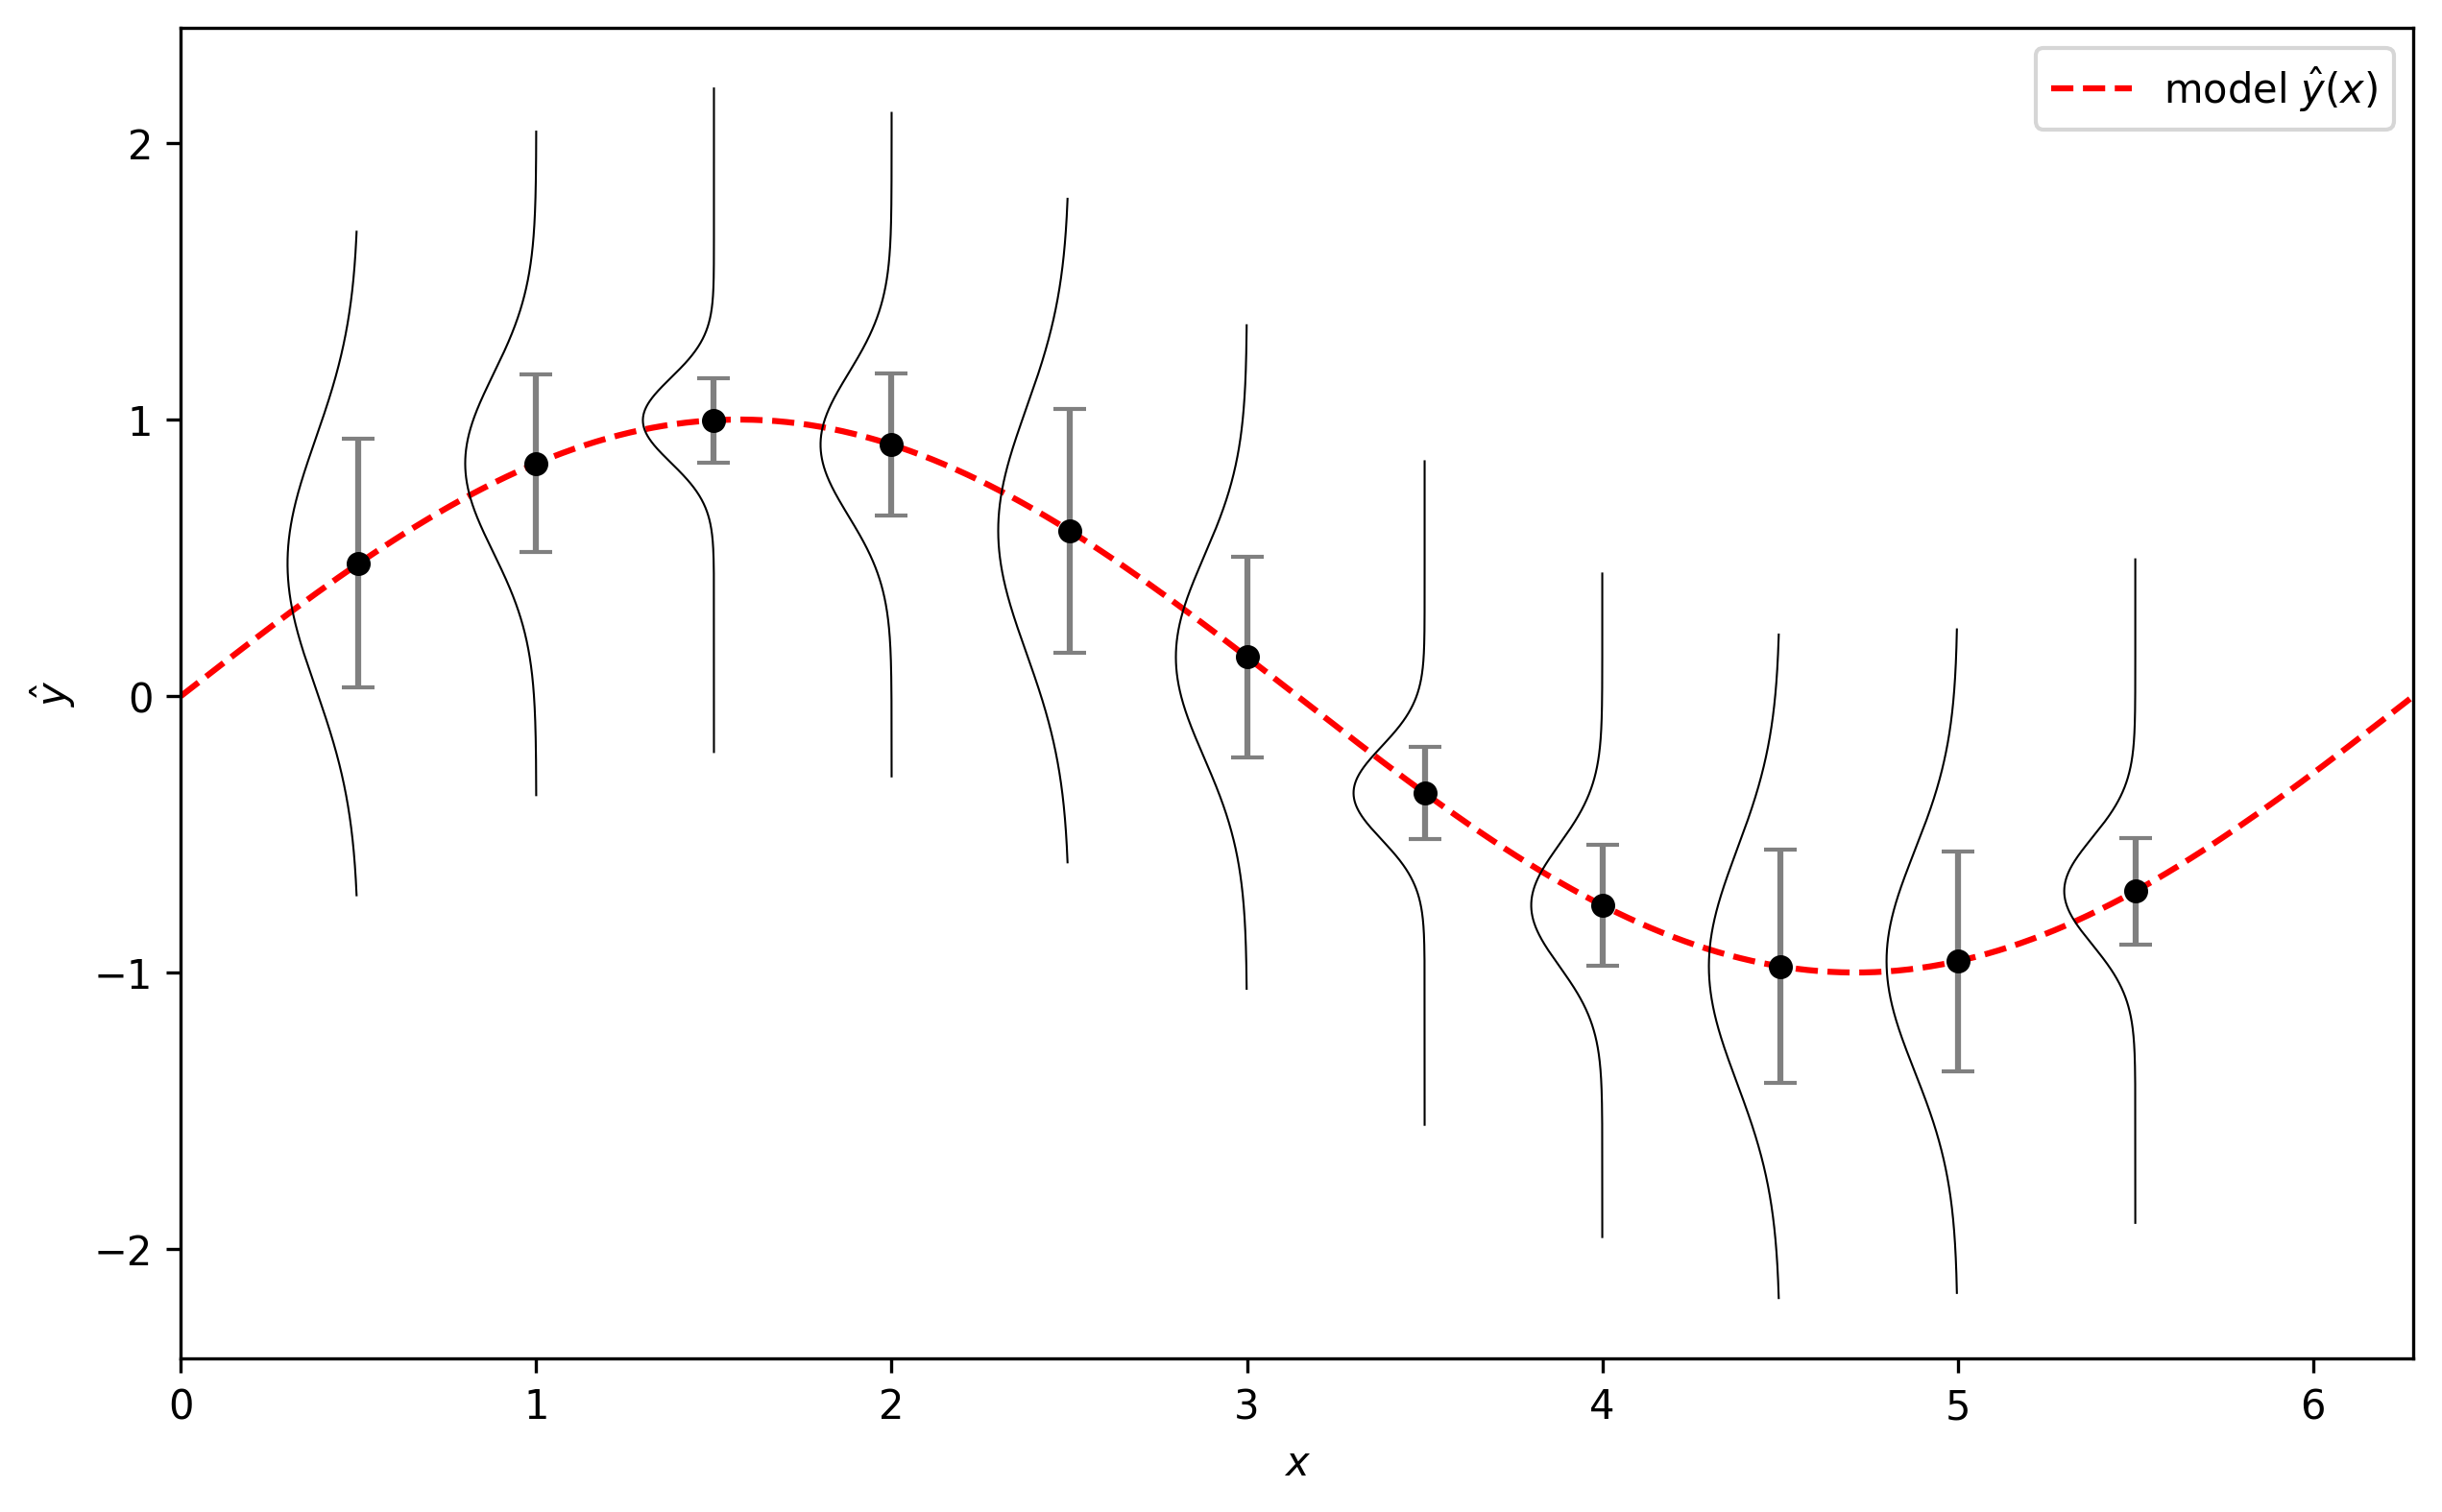
\includegraphics[width=12cm] {model}
\end{figure}

Suppose our model is correct. Then, for every point $ x_i $, we would expect the distribution of our observed $ y_i $ to be Gaussian with mean $ \hat{y}(\vec{a}, x_i) $ and variance $ \sigma_i^2 $. In other words,
\begin{equation}
		y_i \sim N\left(\hat{y}(\vec{a}, x_i) , \sigma_i^2\right)
\end{equation}
If we ``normalize" the random variable $ y_i $,
\begin{equation}
		\frac{y_i - \hat{y}(\vec{a}, x_i) }{\sigma_i} = N(0,1) = X_i
\end{equation}
Defining $ X_i $ to be i.i.d standard normal like in the previous section,
\begin{equation}
		\sum_n 	\left(\frac{y_i - \hat{y}(\vec{a}, x_i) }{\sigma_i}\right)^2 = \sum_i X_i^2 = \chi^2_k
\end{equation}
Thus we were justified in calling \ref{eq:chi2} $\chi^2$. But what is the number of degrees of freedom $ k $? 

Each data point represents a distinct degree of freedom, so with $ n $ data points, we have $ n $ degrees of freedom. However, our model with $ m $ fit parameters uniquely determines $ m $ degrees of freedom. 

In other words, given $ m $ fit parameters: if we know the first $ n-m $ values of $ y_i $, then without loss of generality, we must know the last $ m $ values of $ y_i $ because these are the values such that $ \chi^2 $ is minimized with respect to our model. Therefore, the Chi-squared distribution has $ k=n-m $ degrees of freedom.\footnote{The assumption that our model is a linear combination of functions (\ref{eq:linear}) is critical! If we use an arbitrary model, we can not generally say that there are $n-m $ dof.} 

Now, we define the reduced Chi-squared value to be,
\begin{equation}
		\chi^2_r =\frac{\chi^2}{\nu}; \quad\nu = \text{degrees of freedom}
\end{equation}

Recall that we found (\ref{eq:mean}) the expectation value of $ \chi^2_r $ to be 1. This means that if our model correctly describes the observed data, we would not expect the value of $ \chi^2_r $ to be as small as possible. Instead we expect $ \chi^2_r  =1 $\footnote{Notice that the variance per degree of freedom is also constant (\ref{eq:var}).}. 

If $ \chi^2_r>1 $, it is likely that the model is incorrect or that the fit parameters do not accurately describe the data.

\begin{figure}[H]
	\centering
	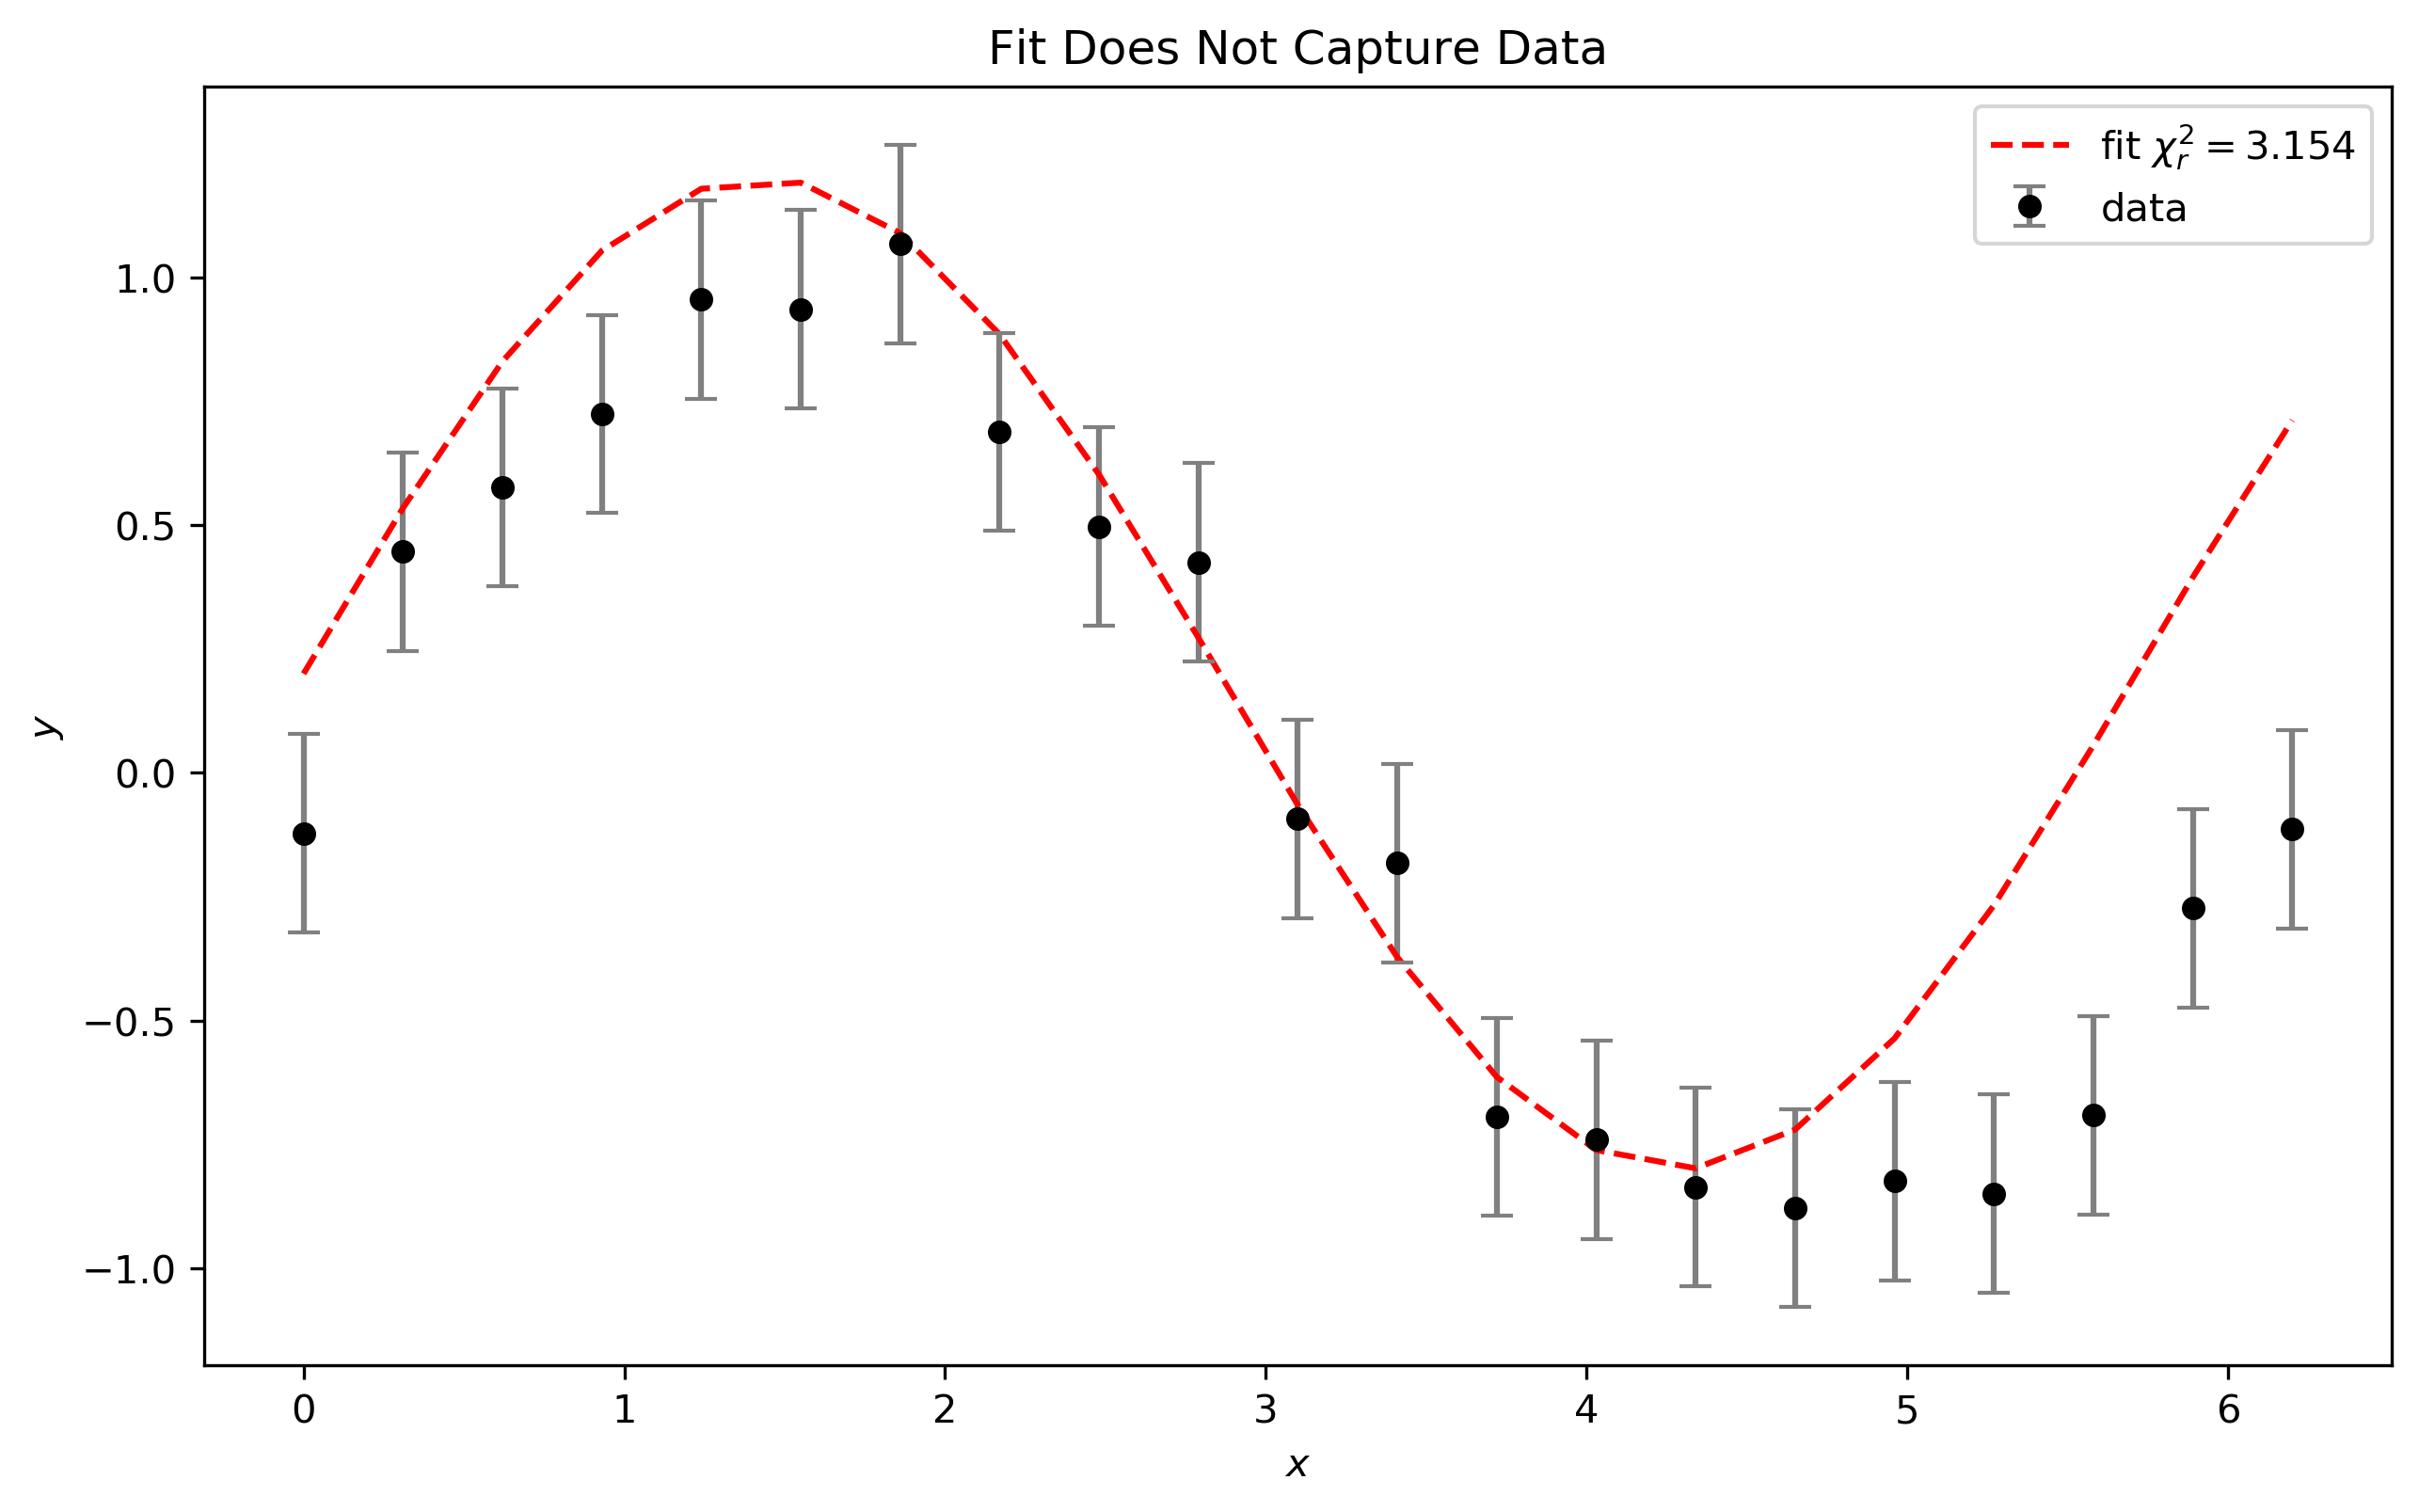
\includegraphics[width=12cm] {bad}
\end{figure}

If $\chi^2_r<1$, it is possible that the data is over fitted: there are too many degrees of freedom in the model and we are fitting noise.

\begin{figure}[H]
	\centering
	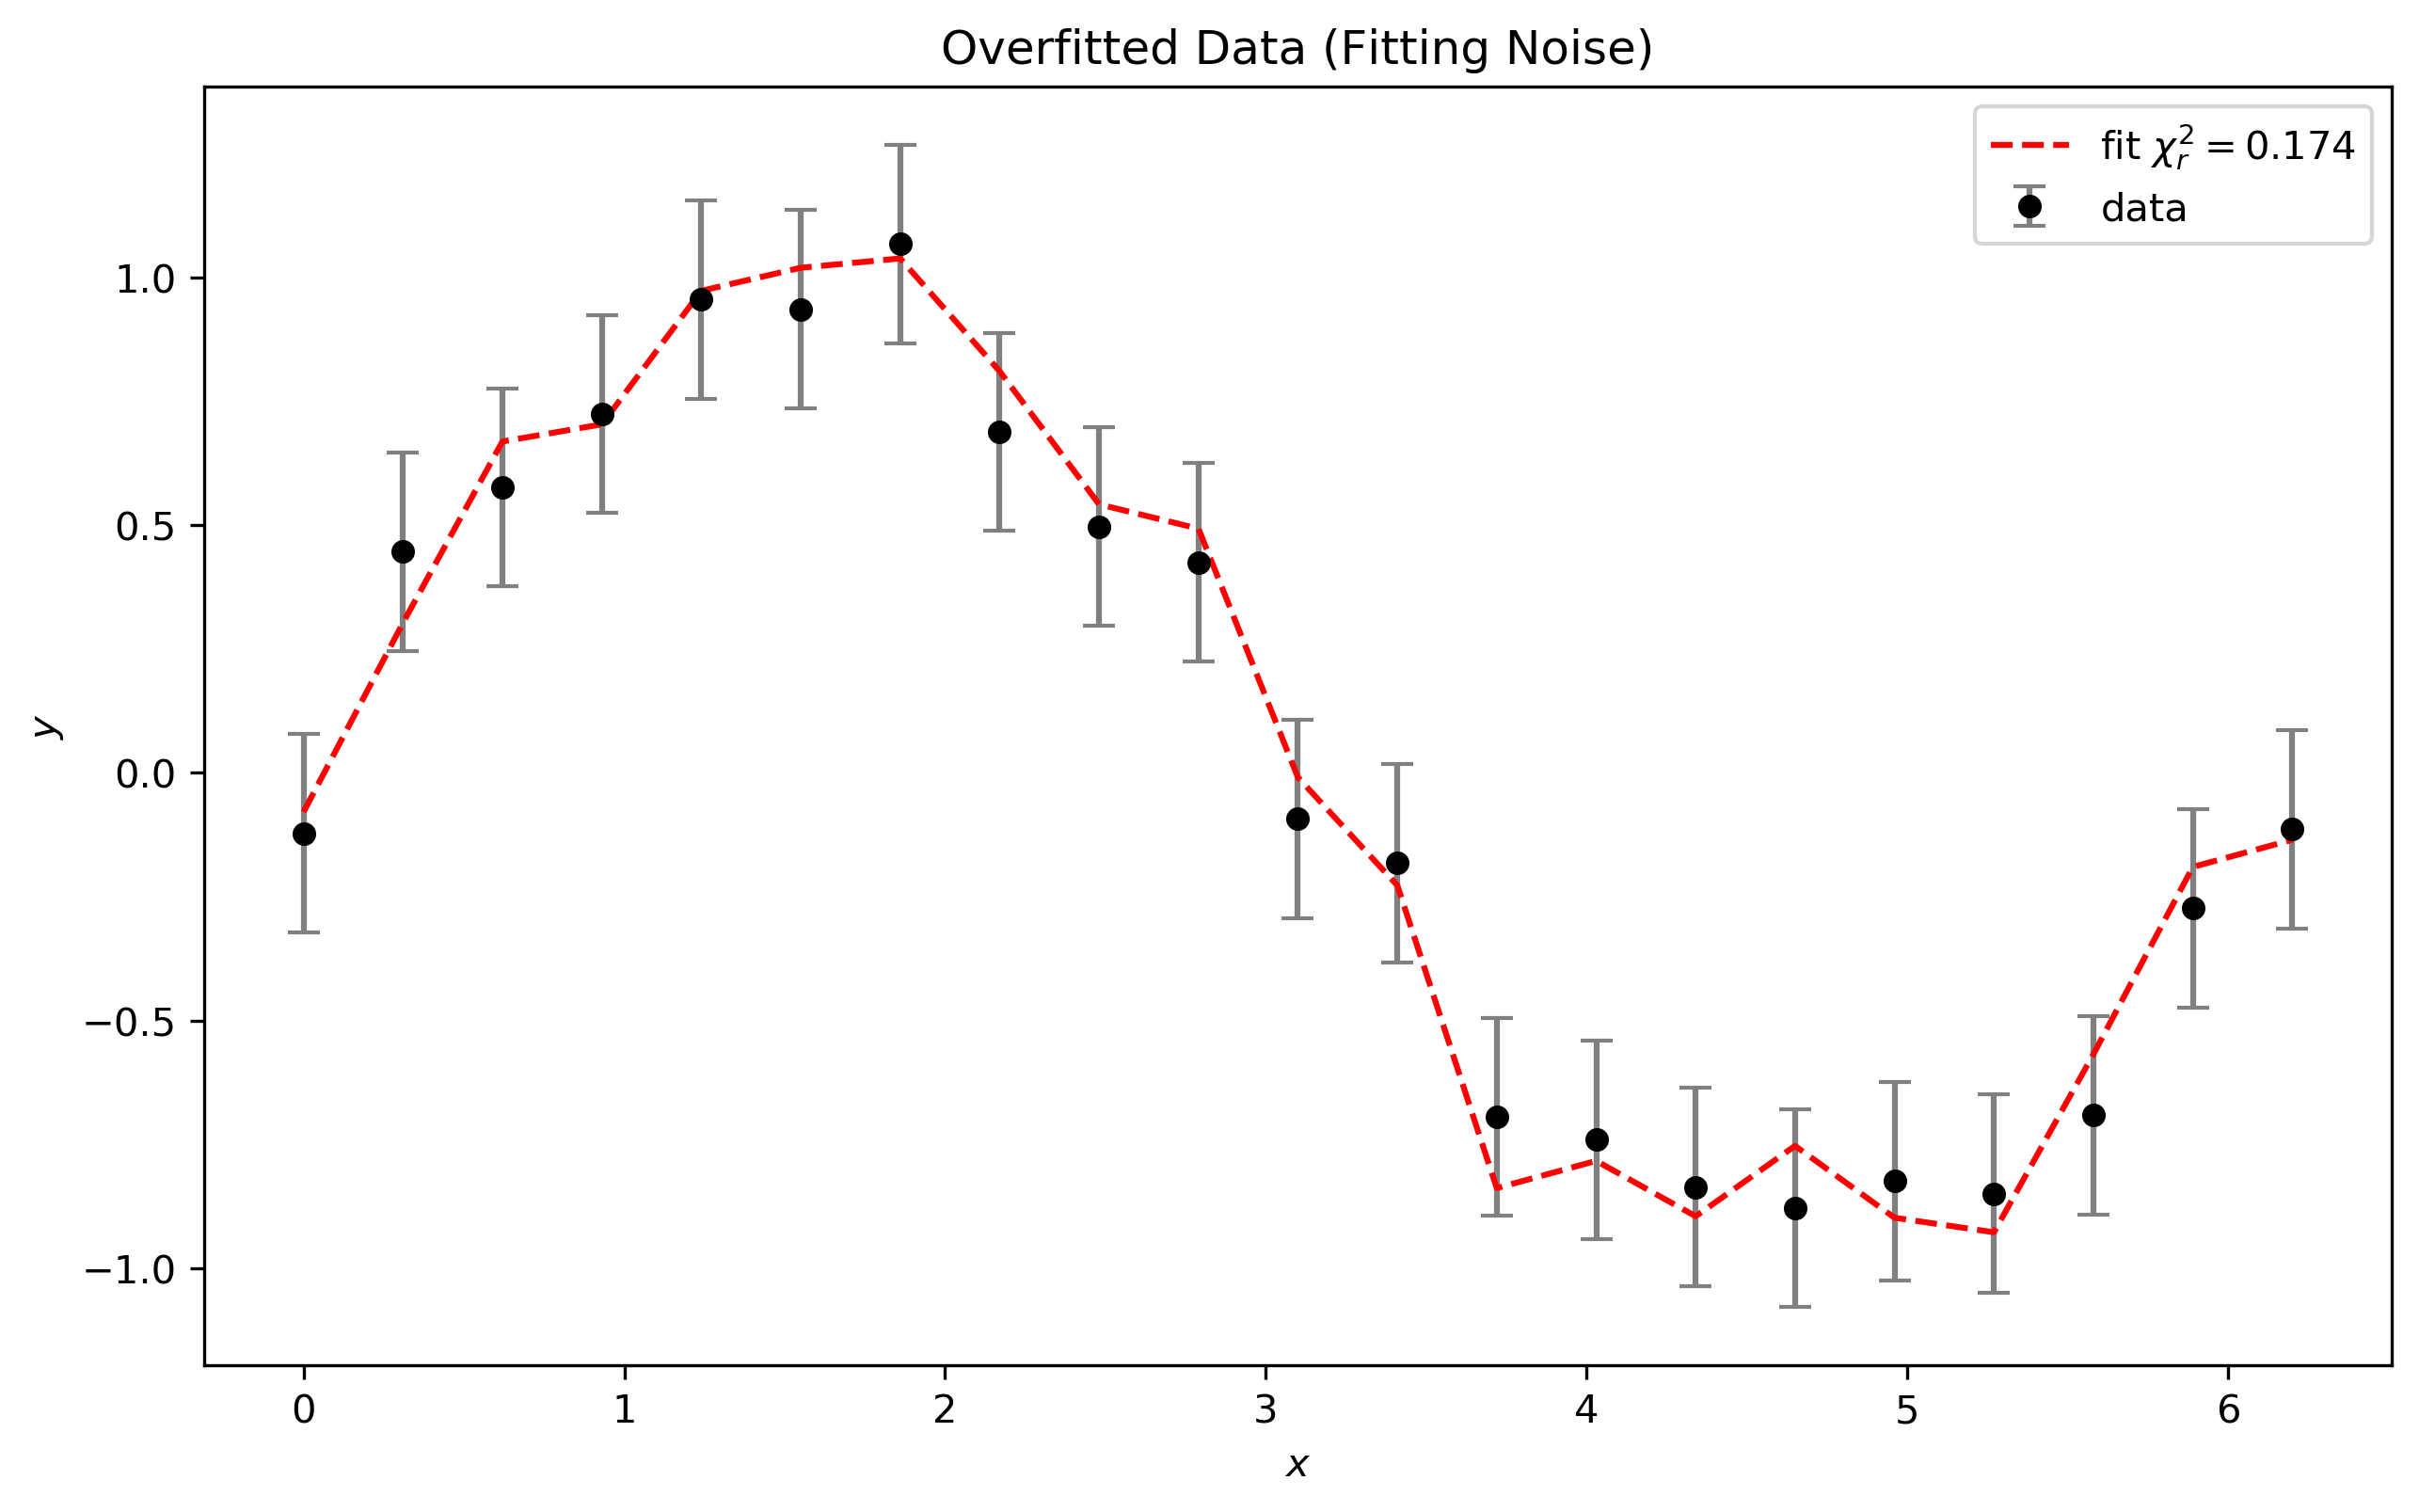
\includegraphics[width=12cm] {over}
\end{figure}

Generally, over fitting is not so dramatic. More subtly, the fit parameters will deviate from their true values in order to account for noise.

Another cause for $\chi^2_r<1$ is if the data uncertainties are overestimated.
\begin{figure}[H]
	\centering
	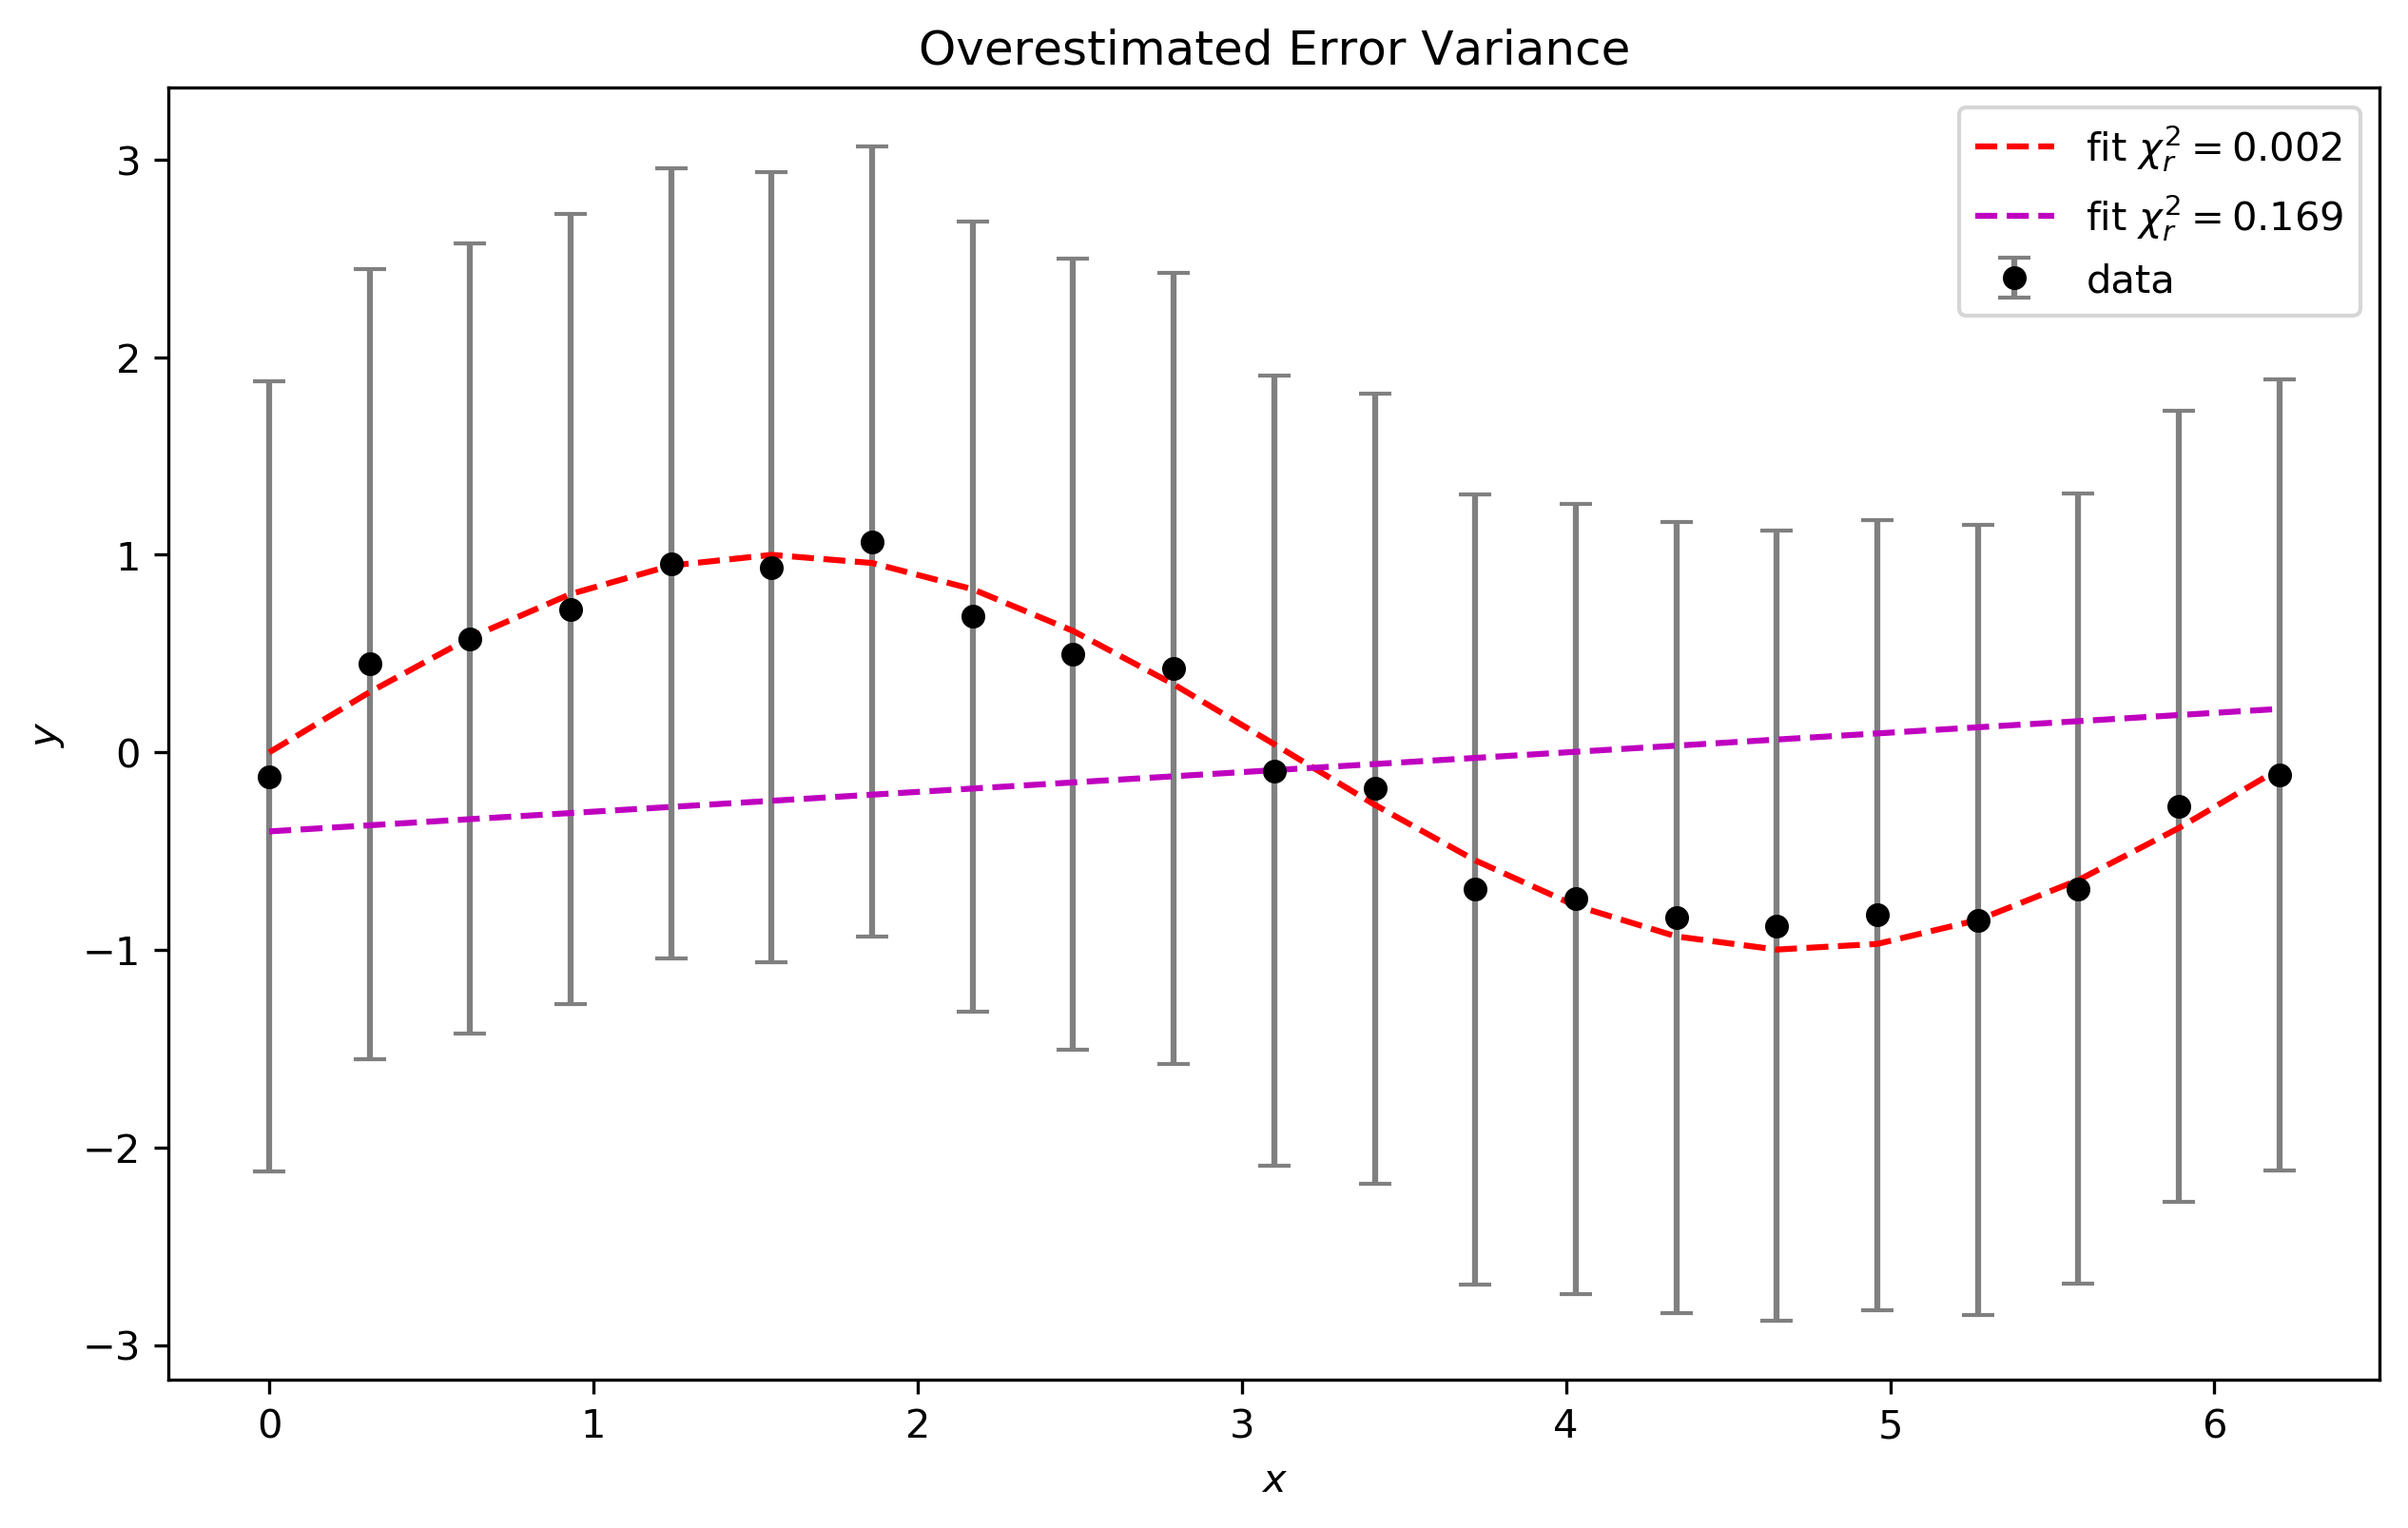
\includegraphics[width=12cm] {var}
\end{figure} 
Here, the measurement uncertainties are so large that the fit is not longer meaningful. 

A rule of thumb for the reduced Chi-squared test is that for a good fit,
\begin{equation}
		0.8 < \chi^2_r < 1.5
\end{equation}


\subsection{Pearson's Chi-Squared Test}

\begin{figure}[H]
	\centering
	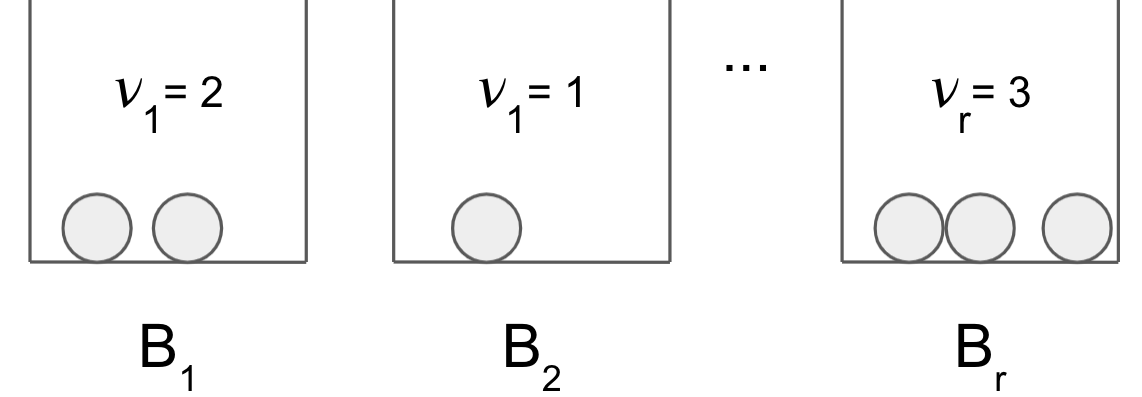
\includegraphics[width=8cm] {boxes}
\end{figure}

Suppose we throw $ n $ balls at $ r $ boxes $ B_i $. The probability of any single ball landing in box $B_i $ is $ p_i $ and independent of any other ball. After all of the balls have been thrown, we observe each box contains $ \nu_i $ balls so that,
\begin{equation}
		\sum_{i=1}^r \nu_i = n
\end{equation}
Given that we observe $ \nu_i $, we want to determine if $ p_i $ is a good model.  The probability of observing $\nu_i$ is given by the multinomial distribution. While we can make use of this fact, another approach is to use Pearson's theorem.

\begin{theorem}[Pearson]
	\begin{equation}
			\sum_{i=1}^r \frac{(\nu_i-np_j)^2}{np_j} \xrightarrow{n\text{ large}} \chi^2_{r-1}
	\end{equation}
	The random variable on the LHS is called the Pearson's Chi-squared variable and converges in distribution (large n) to the Chi-squared distribution with one less degree of freedom.
\end{theorem}

A rigorous treatment of Pearson's theorem is a bit involved, but here I shall present some intuition (this is not a proof!). 

We can define the indicator variable,
\begin{equation}
		 I(X_i\in B_j) = 
		 \begin{cases}
		 	1, & \text{the i-th ball lands in the j-th box}\\
		 	0, & \text{else}
		 \end{cases}
\end{equation} 

Then, we will find that $ \nu_j = \sum_{i=1}^n I(X_i\in B_j) $\footnote{The sum of $ i $ i.i.d. distributions.} and\footnote{Skipping some work to show that for an indicator $I$,  $E(I) = p $ and $ Var(I) = p(1-p) $},
\begin{equation}
		E(\nu_j) = E\left(\sum_{i=1}^n I(X_i\in B_j)\right) = \sum_n E\left[I(X_i\in B_j)\right] = n p_j
\end{equation}
\begin{equation}
		Var(\nu_j) = Var\left(\sum_{i=1}^n I(X_i\in B_j)\right) = n p_j (1-p_j)
\end{equation}
Thus, by the central limit theorem,
\begin{equation}
		\frac{\nu_j - n E(\nu_j)}{\sqrt{n Var(\nu_j)}} = \frac{\nu_j - np_j}{\sqrt{np_j(1-p_j)}} \rightarrow N(0,1)
\end{equation}
\begin{equation}
		\frac{\nu_j - np_j}{\sqrt{np_j}} \rightarrow \sqrt{1-p_j}N(0,1) = N(0, 1-p_j) \approx N(0,1)
\end{equation}
Thus,
\begin{equation}
		\frac{(\nu_j - np_j)^2}{np_j} \rightarrow N(0,1)^2
\end{equation}
We would expect summing over the $ r $ boxes to obtain $ \chi^2_r $. However, notice that $ \nu_i $ are not independent. Because $ \sum_r \nu_i = n $, the system has one less degree of freedom (i.e. if we know the first $ r-1 $ values of $\nu_i$, then we must know $ \nu_r $). The fact that $\nu_i$ are not independent is a major oversight and determining $ \sum_r X_i^2 $ is not so simple!

Regardless, we have now shown some intuition for why Pearson's Chi-squared value should converge to $ \chi^2_{r-1} $. Finally, we can use this relation to perform a $ p $-test for our hypothesis. 

For example, suppose a system has 6 degrees of freedom and we find that (where $ O_i $ are the observed values for each category and $ E_i $ are the expected values for each category),
\begin{equation}
		\chi^2 = \sum_{i=1}^6 \frac{(O_i-E_i)^2}{E_i} = 12.44
\end{equation}
\begin{figure}[H]
	\centering
	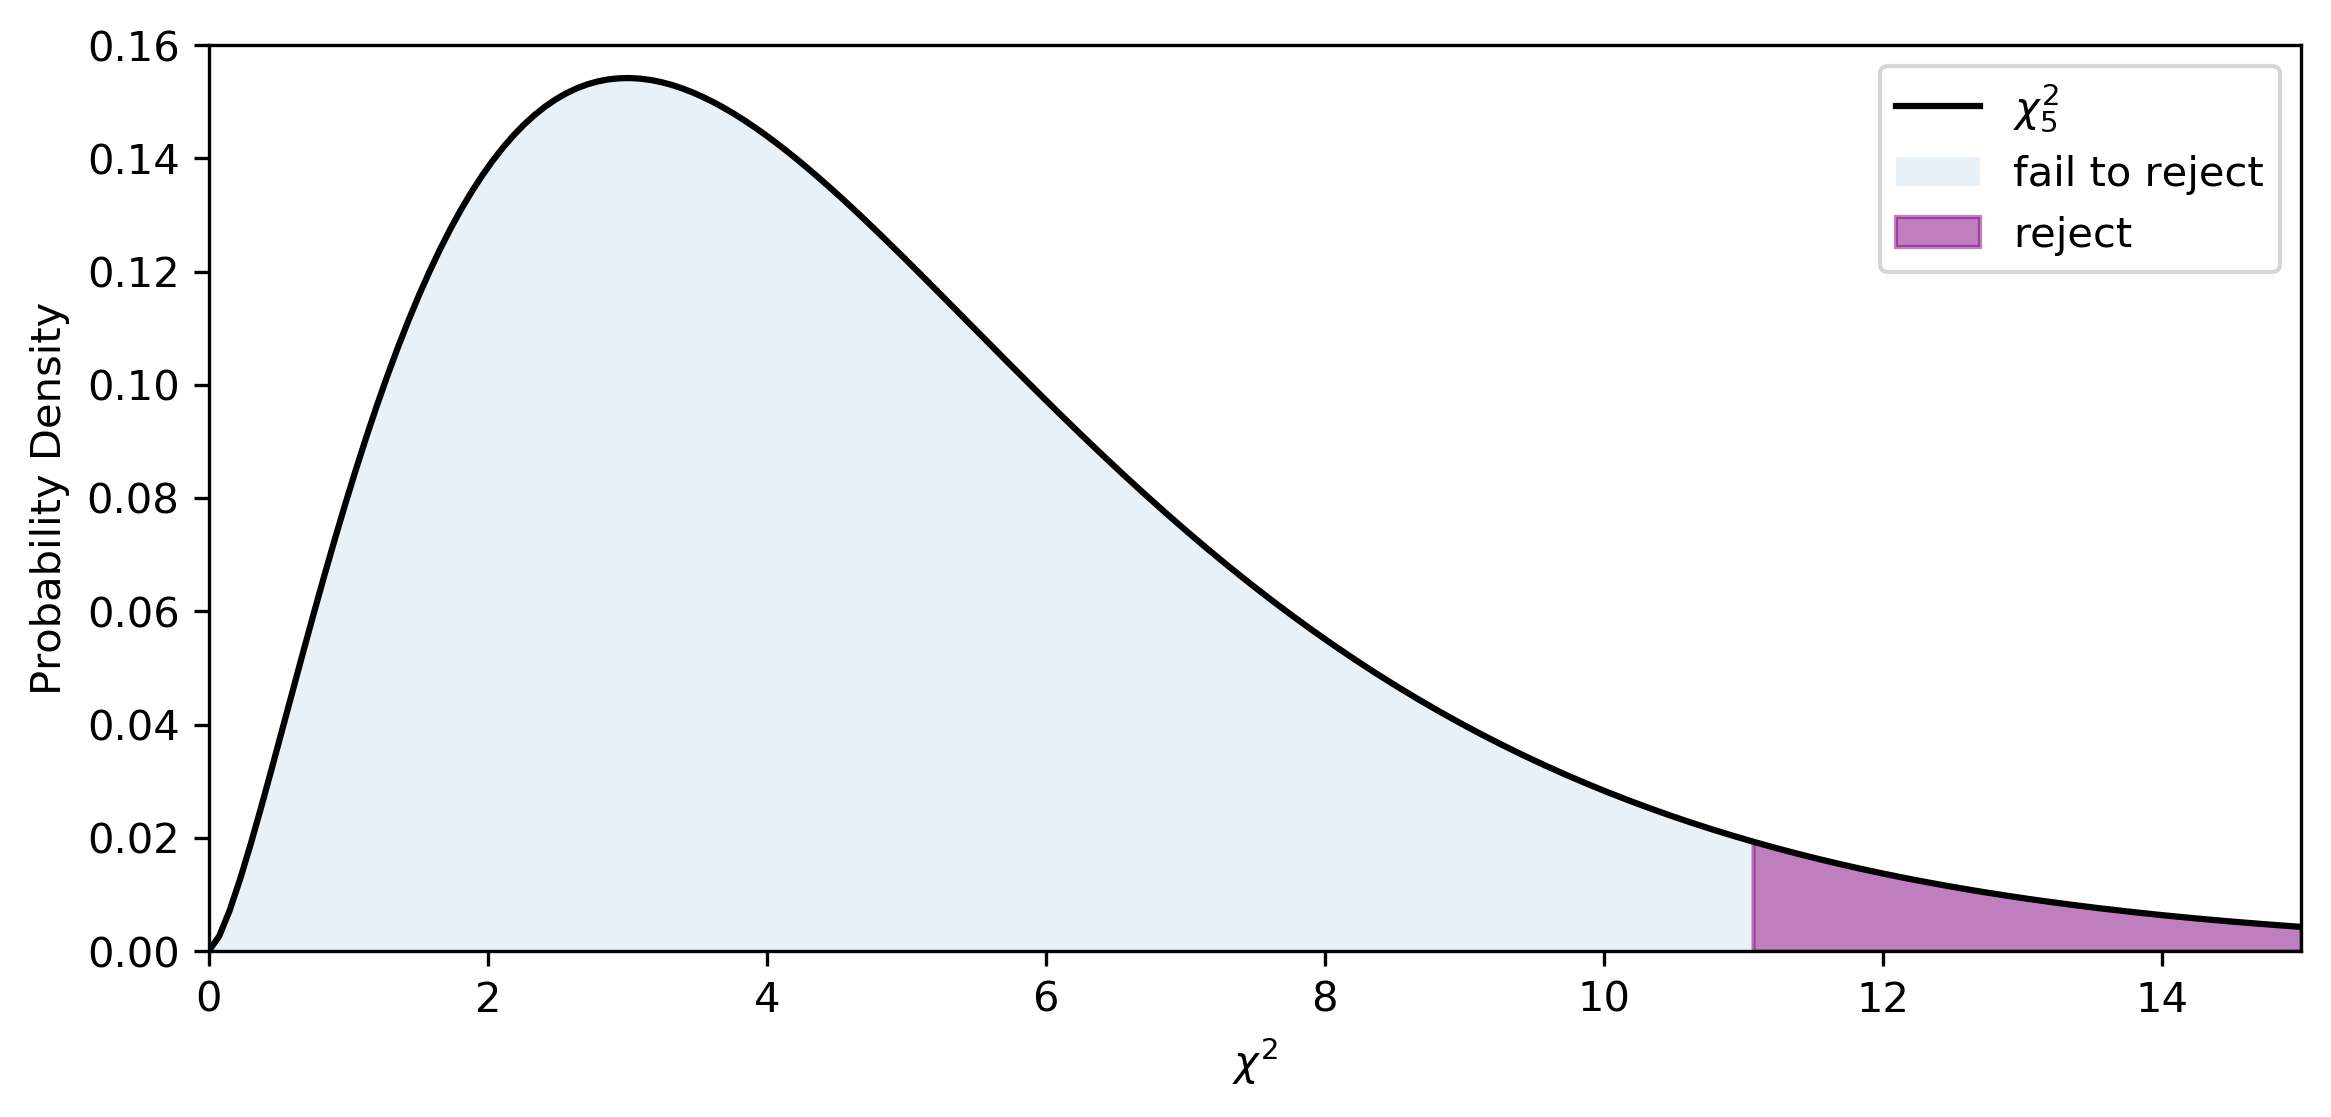
\includegraphics[width=15cm] {critical}
\end{figure}

For a $\chi^2_{k=5}$ distribution with a confidence interval of $ 0.95 $, the critical value is 11.07. This means that there is a 5\% chance of observing a $\chi^2$ greater than 11.07. 

In this case, $ 12.44>11.07 $, we reject our null hypothesis and claim our model is incorrect. If instead, $ \chi^2 < 11.07 $, we fail to reject the null hypothesis.
	
\end{document}